This chapter is dedicated to the implementation related details of the models discussed in the previous chapters. In order to capture and thereafter execute the conceptual model discussed previously, a variety of mechanisms and software implementations were required. Details related to those implementations and the justifications for the corresponding decisions and choices are included and elaborated in this chapter.

\section{Capturing of Data}

In order to assess the behaviour of a system, collection of relevant and accurate data is a must. For the purposes of this study, a number of readings were collected over a period of more than 30 days. Data capturing routines were implemented using Python programming language. Python was chosen as the language for implementation, due to its simple and expressive syntax, support for extended arithmetic operations such as power and floor division and the comparatively higher availability of various modules and extension \acrfull{api}s.

During the capturing of data, reading and transformation concerns such as fast and easy access, was taken into consideration. Hence, the data being captured were stored in \ilcode{JSON} initially. \acrfull{json} was chosen as the storage structure due to the simplistic nature and flexible support for that format awarded by python. Further, the data that was captured was processed later as a batch and written into a database in MongoDB. MongoDB was chosen again due to the freedom interfacing with python and freedom and performance in querying.

As discussed previously, this study focuses on both the internal and the external environments, under the constraints of

\begin{itemize}
    \item Technological Feasibility
    \item Portability
    \item Economical Feasibility (i.e. Cost effectiveness)
\end{itemize}

There are certain phenomenon such as software and hardware interrupts, context switches and so forth, which are deemed to be sufficiently random by certain applications, such as \ilcode{/dev/random} and \ilcode{/dev/urandom} in Unix Systems \cite{web_linux_rand_urand}.

Python has a module named \ilcode{psutil} which is designed to capture the CPU and RAM metrics and so forth. A python routine was implemented which consumes these functions from the \ilcode{psutil} which is attached as appendix \ref{adx:grabber}. When collecting data, the following functions in \ilcode{psutil} were invoked.

\begin{enumerate}
    \item \ilcode{psutil.cpu\_stats()} - Collects CPU statistics including hardware and software interrupt counts, number of system calls and number of context switches
    \item \ilcode{psutil.sensors\_temperatures(1)} - Core temperature metrics of the CPU
    \item \ilcode{psutil.virtual\_memory()} - Various counts of memory of the computer including but not limited to available memory, used memory, cached memory and so forth
    \item \ilcode{psutil.disk\_usage("/")} - Disk usage of a given mount point (in linux)
\end{enumerate}

A sample of such a result, represented as a MongoDB document is indicated in the code listing below (Listing \ref{lst:samp_cpu_dat}).

\begin{code}
    \begin{minted}[breaklines]{json}
        {
            "_id" : 1555041606,
            "sdiskusage" : {
                "total" : NumberLong(51471126528),
                "used" : NumberLong(42555625472),
                "percent" : 87.1,
                "free" : NumberLong(6277283840)
            },
            "scpustats" : {
                "interrupts" : 2092921,
                "soft_interrupts" : 1537679,
                "syscalls" : 0,
                "ctx_switches" : 4502862,
                "temperature" : {
                    "nouveau" : [ 
                        [ 
                            "", 
                            120.2, 
                            203.0, 
                            221.0
                        ]
                    ],
                    "acpitz" : [ 
                        [ 
                            "", 
                            123.8, 
                            null, 
                            null
                        ]
                    ],
                    "coretemp" : [ 
                        [ 
                            "Core 0", 
                            111.2, 
                            221.0, 
                            221.0
                        ], 
                        [ 
                            "Core 1", 
                            111.2, 
                            221.0, 
                            221.0
                        ]
                    ]
                }
            },
            "svmem" : {
                "available" : 1991725056,
                "used" : 1804324864,
                "cached" : 1569783808,
                "percent" : 51.9,
                "free" : 391614464,
                "inactive" : 837197824,
                "active" : NumberLong(2480824320),
                "shared" : 48029696,
                "total" : NumberLong(4140666880),
                "slab" : 303345664,
                "buffers" : 374943744
            }
        }
    \end{minted}
    \caption{Example of CPU data collected into a MongoDB document}
    \label{lst:samp_cpu_dat}
\end{code}

Two systems were monitored with this routine where one system was running at idle and the other was being used by a software developer. A total of 1838879 data documents from idle system and 1999681 data documents from the working system, which maps to each second of a mix of continuous and noncontinuous time frames were collected and, each document was assigned with the corresponding epoch timestamp\footnote{The Unix epoch (or Unix time or POSIX time or Unix timestamp) is the number of seconds that have elapsed since January 1, 1970 (midnight UTC/GMT), not counting leap seconds (in ISO 8601: 1970-01-01T00:00:00Z).\cite{web_epoch_def}} as the ID.

\section{Distillation and Transformation}

The metrics obtained in the previous step were observed initially and the numeric values were extracted. During the extraction the values that were potential seeds, the primary concern was those values to demonstrate variations over time and the \textit{rate of change} to be as high as possible. In order to do a systematic comparison, two systems were monitored simultaneously, that which both of them were having the same version of the same operating system running, one running at idle, and the other one being used by a software developer which engages in various software development work. Then, the metrics were evaluated for their quality as seeds for the transformation process.

The distillation was mainly based on statistical analysis and visualisation of data points using graphs. for the primary filtering of data items, values for each metric for ten seconds were visually inspected for their appearances of suitable variations. This was repeated over a 100 different samples and then the observations were tallied. A sample of such observations is graphically depicted below (Table \ref{tab:c4_ten_sec_cpu_dat_idle}).

\afterpage{\clearpage}
\begin{sidewaystable}[h]
    \small
    \resizebox{\textwidth}{!}{\begin{tabular}{|l|c|c|c|c|c|c|c|c|c|c|}
        \hline
        \textbf{sdiskusage.percent} & 83.5 & 83.5 & 83.5 & 83.5 & 83.5 & 83.5 & 83.5 & 83.5 & 83.5 & 83.5 \\ \hline
        \textbf{sdiskusage.free} & 8080375808 & 8080375808 & 8080375808 & 8080375808 & 8080375808 & 8080375808 & 8080375808 & 8080375808 & 8080375808 & 8080375808 \\ \hline
        \textbf{scpustats.interrupts} & 62734861 & 62735347 & 62735834 & 62736290 & 62736681 & 62737063 & 62737443 & 62737847 & 62738260 & 62738686 \\ \hline
        \textbf{scpustats.soft\_interrupts} & 32646241 & 32646570 & 32646907 & 32647196 & 32647394 & 32647585 & 32647759 & 32647938 & 32648143 & 32648406 \\ \hline
        \textbf{scpustats.syscalls} & 0 & 0 & 0 & 0 & 0 & 0 & 0 & 0 & 0 & 0 \\ \hline
        \textbf{scpustats.ctx\_switches} & 75075959 & 75076482 & 75077126 & 75077759 & 75078166 & 75078568 & 75078967 & 75079360 & 75079786 & 75080366 \\ \hline
        \textbf{scpustats.temperature.nouveau.0.0} &  &  &  &  &  &  &  &  &  &  \\ \hline
        \textbf{scpustats.temperature.nouveau.0.1} & 118.4 & 118.4 & 118.4 & 118.4 & 118.4 & 118.4 & 118.4 & 118.4 & 116.6 & 118.4 \\ \hline
        \textbf{scpustats.temperature.nouveau.0.2} & 203.0 & 203.0 & 203.0 & 203.0 & 203.0 & 203.0 & 203.0 & 203.0 & 203.0 & 203.0 \\ \hline
        \textbf{scpustats.temperature.nouveau.0.3} & 221.0 & 221.0 & 221.0 & 221.0 & 221.0 & 221.0 & 221.0 & 221.0 & 221.0 & 221.0 \\ \hline
        \textbf{scpustats.temperature.acpitz.0.0} &  &  &  &  &  &  &  &  &  &  \\ \hline
        \textbf{scpustats.temperature.acpitz.0.1} & 120.2 & 120.2 & 120.2 & 120.2 & 120.2 & 120.2 & 120.2 & 120.2 & 120.2 & 120.2 \\ \hline
        \textbf{scpustats.temperature.acpitz.0.2} & None & None & None & None & None & None & None & None & None & None \\ \hline
        \textbf{scpustats.temperature.acpitz.0.3} & None & None & None & None & None & None & None & None & None & None \\ \hline
        \textbf{scpustats.temperature.coretemp.0.0} & Core 0 & Core 0 & Core 0 & Core 0 & Core 0 & Core 0 & Core 0 & Core 0 & Core 0 & Core 0 \\ \hline
        \textbf{scpustats.temperature.coretemp.0.1} & 105.8 & 104.0 & 104.0 & 104.0 & 104.0 & 104.0 & 104.0 & 104.0 & 104.0 & 104.0 \\ \hline
        \textbf{scpustats.temperature.coretemp.0.2} & 221.0 & 221.0 & 221.0 & 221.0 & 221.0 & 221.0 & 221.0 & 221.0 & 221.0 & 221.0 \\ \hline
        \textbf{scpustats.temperature.coretemp.0.3} & 221.0 & 221.0 & 221.0 & 221.0 & 221.0 & 221.0 & 221.0 & 221.0 & 221.0 & 221.0 \\ \hline
        \textbf{scpustats.temperature.coretemp.1.0} & Core 1 & Core 1 & Core 1 & Core 1 & Core 1 & Core 1 & Core 1 & Core 1 & Core 1 & Core 1 \\ \hline
        \textbf{scpustats.temperature.coretemp.1.1} & 105.8 & 104.0 & 104.0 & 104.0 & 104.0 & 105.8 & 105.8 & 105.8 & 105.8 & 105.8 \\ \hline
        \textbf{scpustats.temperature.coretemp.1.2} & 221.0 & 221.0 & 221.0 & 221.0 & 221.0 & 221.0 & 221.0 & 221.0 & 221.0 & 221.0 \\ \hline
        \textbf{scpustats.temperature.coretemp.1.3} & 221.0 & 221.0 & 221.0 & 221.0 & 221.0 & 221.0 & 221.0 & 221.0 & 221.0 & 221.0 \\ \hline
        \textbf{svmem.available} & 2684878848 & 2684878848 & 2684891136 & 2684899328 & 2684899328 & 2684899328 & 2684899328 & 2684899328 & 2684899328 & 2684899328 \\ \hline
        \textbf{svmem.used} & 1117835264 & 1117835264 & 1117835264 & 1117835264 & 1117835264 & 1117835264 & 1117835264 & 1117835264 & 1117835264 & 1117835264 \\ \hline
        \textbf{svmem.cached} & 1331859456 & 1331859456 & 1331859456 & 1331859456 & 1331859456 & 1331859456 & 1331859456 & 1331859456 & 1331859456 & 1331859456 \\ \hline
        \textbf{svmem.percent} & 35.2 & 35.2 & 35.2 & 35.2 & 35.2 & 35.2 & 35.2 & 35.2 & 35.2 & 35.2 \\ \hline
        \textbf{svmem.free} & 1271947264 & 1271947264 & 1271947264 & 1271947264 & 1271947264 & 1271947264 & 1271947264 & 1271947264 & 1271947264 & 1271947264 \\ \hline
        \textbf{svmem.inactive} & 662401024 & 662401024 & 662409216 & 662409216 & 662409216 & 662409216 & 662409216 & 662409216 & 662409216 & 662409216 \\ \hline
        \textbf{svmem.active} & 1879252992 & 1879252992 & 1879257088 & 1879252992 & 1879252992 & 1879252992 & 1879252992 & 1879252992 & 1879252992 & 1879252992 \\ \hline
        \textbf{svmem.shared} & 41353216 & 41353216 & 41353216 & 41353216 & 41353216 & 41353216 & 41353216 & 41353216 & 41353216 & 41353216 \\ \hline
        \textbf{svmem.total} & 4140666880 & 4140666880 & 4140666880 & 4140666880 & 4140666880 & 4140666880 & 4140666880 & 4140666880 & 4140666880 & 4140666880 \\ \hline
        \textbf{svmem.slab} & 231829504 & 231829504 & 231829504 & 231829504 & 231829504 & 231829504 & 231829504 & 231829504 & 231829504 & 231829504 \\ \hline
        \textbf{svmem.buffers} & 419024896 & 419024896 & 419024896 & 419024896 & 419024896 & 419024896 & 419024896 & 419024896 & 419024896 & 419024896 \\ \hline
    \end{tabular}}
    \caption{Tabulation of CPU statistics within a 10 second window for observation (Idle Device)}
        \label{tab:c4_ten_sec_cpu_dat_idle}
\end{sidewaystable}

As per the table, it is obvious that the following parameters demonstrate a rapid change.

\begin{enumerate}
    \item Number of Context Switches
    \item Number of Hardware Interrupts
    \item Number of Software Interrupts
\end{enumerate}

Other metrics such as CPU core temperatures, disk usage and all are demonstrating no changes at all in most cases. The same was observable in other windows also for the static/idle system. So, it has concluded to utilise a combination of these variables as the inputs to the seed generator.

\newpage

\subsection{Floating Point Conversion Algorithm}
The author has taken note on the fact that the floating point algorithm is quite simple to implement and execute. More importantly, the algorithm could be implemented in such a way that it takes arbitrary values for its primary parameters $E$ and $m$. Hence, this algorithm was implemented using python, to take a decimal number as a string and to convert it to a floating point number of arbitrary exponent and mantissa size. Python was chosen as the language to implement, primarily due to its expressive syntax and native support for certain operations on arrays and lists such as map-reduce functions, \textit{for-each} loop, type conversions and string manipulation operations. The algorithm which was initially implemented is as the code listing outlined below (see Listing \ref{lst:py_class_float}).

The intention of implementing this algorithm was to closely analyse the behaviour of the bit strings of the numbers when they are converted to floating point. Upon the analysis, the mantissa conversion routine was identified to be a suitable component, which could be used at the core of the proposed algorithm for generation. This routine is as outlined below (listing \ref{lst:float_mantissa_subr}).

\begin{code}
    \begin{minted}[breaklines,tabsize=2]{py}
        # Resolution of float
		f = n1[1]
		f = [int(e.encode('ascii')) for e in f]

		zero = [0] * len(f)

		sig = []

		decPosFound = decPos > -1

		while True:
			if f == zero:
				break
			
			[of, f] = self.__arrayTimes2(f)

			if not decPosFound:
				if of == 1:
					decPosFound = True
				else:
					decPos -= 1
			
			if len(sig) >= (m - decPos):
				break

			sig.append(of)
    \end{minted}
    \caption{Mantissa Derivation Subroutine of Floating Point Converter}
    \label{lst:float_mantissa_subr}
\end{code}

\subsection{Proposed Algorithm - FloatRAND}

The proposed algorithm implements the mantissa conversion routine at its core, to generate the next bit. All that is provided by this algorithm is a mechanism to utilise a microscopic value (hereafter referred to as seed) to generate random bit stream which are of high statistical quality. This is precisely a state machine that depends on the inputs given and is a One-to-One mapping between the seed and the bit string generated. For an instance,

\[
    0.33_{10} = 0.0101010001111010111\ldots_{2}
\]

where the seed 0.33 into this algorithm will produce $010101000111\ldots$ as the random bit stream. The algorithm is designed in a manner that it takes two arbitrary integers $S_1$ and $S_2$, both of which are 6-7 digits long and the ratio (i.e. $S_1/S_2$) of these are taken as the seed. Now, given a quotient, there are infinitely many number of possible combinations for the numerator and denominator, which all of them are correct. Therefore it is computationally infeasible to determine the exact numerator and denominator pair used to obtain the given quotient. The only possibility is doing an exhaustive brute force on all possible combinations and querying someone who knows the answer who in fact is the challenger himself. If the challenger is not willing to disclose the answer, there is no way that it could be verified. Hence this can be regarded as a non-deterministic problem.

\subsubsection{Algorithmic Details}

Initialisation of the algorithm requires two seeds which are about 6-7 digits long (could be grater) and approximately similar in size. Quotient of these two seeds are used by the core routine to generate bits. Quotient should be obtained to a precision about 20 digits in order to generate bits at the optimum. Larger quotients will generate bit strings which demonstrate better statistical quality, at the cost of lower generation speeds. Precision below 10 digits are not recommended due to the low statistical quality and existence of obvious patterns.

The fractional portion of the quotient is pushed into the seed buffer and then the seed buffer is repeatedly multiplied by two (2) and the overflow of the multiplication will be the next bit. Hence the multiplication of any decimal digit is always less than 20, the overflow will always be either 1 or 0. The generation stops when either the desired length is reached or all digits in the seed buffer becomes 0. This could be graphically depicted as below (figure \ref{fig:floatrand_ex}).

\begin{figure}[h!]
    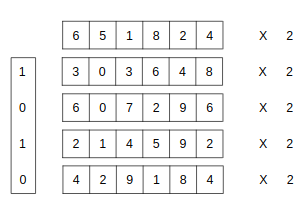
\includegraphics[width=0.7\textwidth]{floatrand_ex.png}
    \centering
    \caption{FloatRAND - Generation}
    \label{fig:floatrand_ex}
\end{figure}

Given the seeds are chosen from random sources, the algorithm provides adequate statistical qualities of randomness which are desired by most of the applications in the personal domain. If the sources of randomness chosen are proven to have the quality attributes of randomness discussed above, the generator shall have the desired security as well, due to the non-deterministic nature of the core.

\subsubsection{Known Weaknesses}

However, the following weaknesses were identified at the initial stage.

\begin{itemize}
    \item Seed and the bit string has a one to one mapping. Hence, an attacker who has the output bit string can generate the seed, but not the random variables.

    \item Seeds with too many zeros, less number of digits (digit count below 7) are generating strings which are of poor quality

    \item Performance depends on the computational resources.

    \item Serial - Each iteration of the core generates only one bit
\end{itemize}


\section{Hardening}